\section{Introduzione}
\subsection{Sistemi di equazioni}
L'algebra lineare è lo studio delle soluzioni di sistemi di equazioni lineari utilizzando spazzi vettoriali.
\begin{example}
Con sistemi di equazioni si intende per esempio:
\begin{enumerate}
    \item \hspace{.3cm} $\begin{rcases*}E_1: x + y = 5 \\ E_2: x + 2y = 6\:\:\end{rcases*} \Rightarrow E_2 - E_1$ (sostituzione): $\begin{cases}y = 5 - 3 = 2 \\ x = 3 - 2 = 1\end{cases}$ \hspace{.2cm} Un unica soluzione.
    \item \hspace{.3cm} $\begin{rcases*}E_1: x + y = 3 \\ E_2: 2x + 2y = 6\:\:\end{rcases*} \Rightarrow E_2 - 2E_1$: 0 = 0.\\\\
    Infatti $E_2 = 2E_1 \Rightarrow$ hanno le stesse soluzioni $\Rightarrow$ $E_{\infty}$ infinite soluzioni.
    \item \hspace{.3cm} $\begin{rcases*}E_1: x + y = 3 \\ E_2: 2x + 2y = 5\:\:\end{rcases*} \Rightarrow E_2 - 2E_1: 0 = -1$ è impossibile infatti $\nexists$ soluzioni comuni.
\end{enumerate}
Possiamo vedere da questi esempi che abbiamo il primo caso con 1 soluzione, il secondo con $\infty$ ed il terzo con 0 soluzioni comuni.
\end{example}

\subsection{Interpretazioni geometrica}
In ogni caso le equazioni $E_1$ ed $E_2$ rappresentano rette su un piano in questo caso a 2 dimensioni, nel caso di questi tre esempi abbiamo che:
\begin{figure}[h!]
    \centering
    \begin{subfigure}{.3\textwidth}
        \centering
        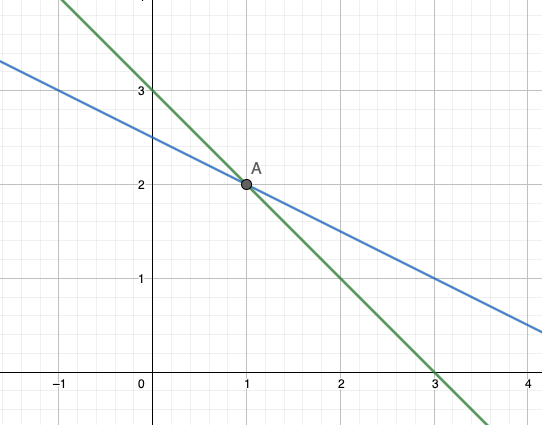
\includegraphics[width=3cm]{images/rette-incidenti.png}
        \caption{1° hanno un punto in comune P=(1,2)}
    \end{subfigure}
    \hfill
    \begin{subfigure}{.3\textwidth}
        \centering
        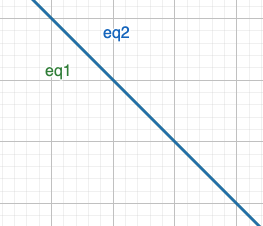
\includegraphics[width=3cm]{images/rette-coincidenti.png}
        \caption{2° coincidono $\Rightarrow \infty$ punti in comune}
    \end{subfigure}
    \hfill
    \begin{subfigure}{.3\textwidth}
        \centering
        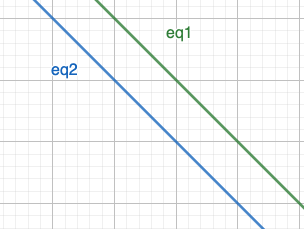
\includegraphics[width=3cm]{images/rette-parallele.png}
        \caption{3° sono parallele  $\Rightarrow \nexists$ punti in comune}
    \end{subfigure}
\end{figure}
\newpage
\subsection{Equazioni a 3 variabili}
Un esempio di equazione a 3 variabili è $x + 2y + 3z = 4$. Ciò crea non una retta ma un piano nello spazio a 3-dimensionale.
Se adesso consideriamo le equazioni viste sopra $E_1$ ed $E_2$ come equazioni a 3 variabili possiamo vedere che essere corrispondo a 2 piano nello spazio ed i punti in comune formano una retta.
\begin{figure}[h!]
    \centering
    \begin{subfigure}{.3\textwidth}
        \centering
        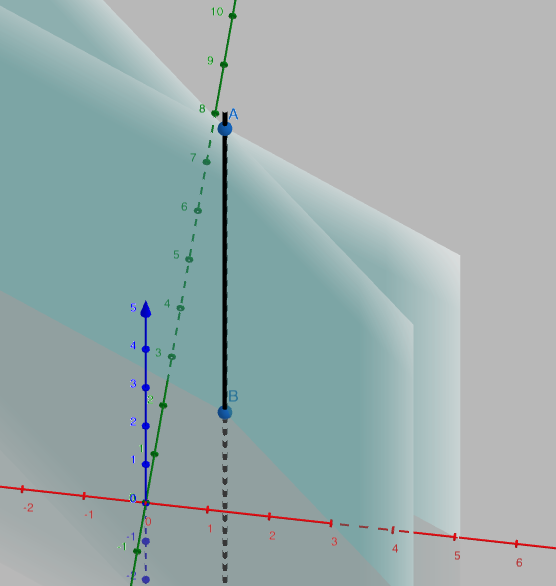
\includegraphics[width=2.5cm]{images/piani-incidenti.png}
        \caption{1° fora una retta}
    \end{subfigure}
    \begin{subfigure}{.3\textwidth}
        \centering
        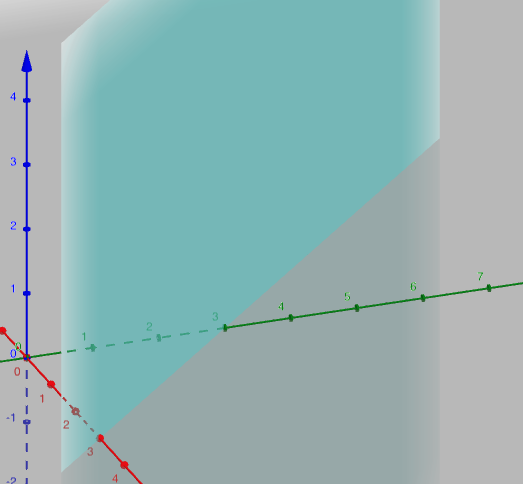
\includegraphics[width=2.5cm]{images/piani-coincidenti.png}
        \caption{2° i due piani coincidono}
    \end{subfigure}
    \begin{subfigure}{.3\textwidth}
        \centering
        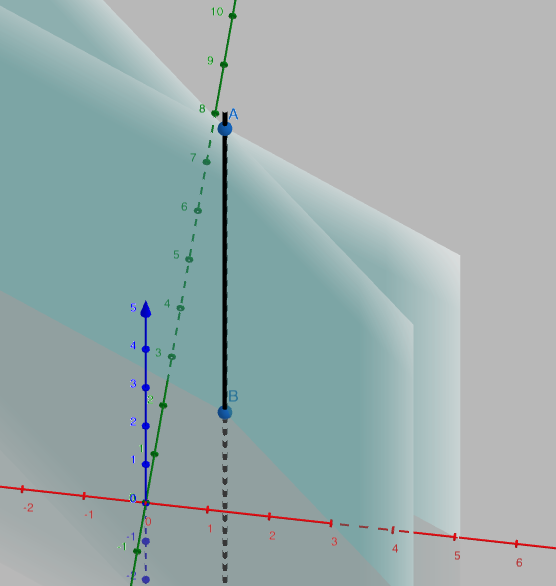
\includegraphics[width=2.5cm]{images/piani-incidenti.png}
        \caption{3° i due piano sono paralleli}
    \end{subfigure}
\end{figure}
Se oltre a $E_1$ ed $E_2$ consideriamo una terza equazione $E_3$ essa corrisponde ad un terzo piano, possiamo vedere esso come può comportarsi intersecandolo con l'intersezione fra $E_1$ ed $E_2$, $E_1 \cap E_2$.
\begin{figure}[h!]
    \centering
    \begin{subfigure}{.3\textwidth}
        \centering
        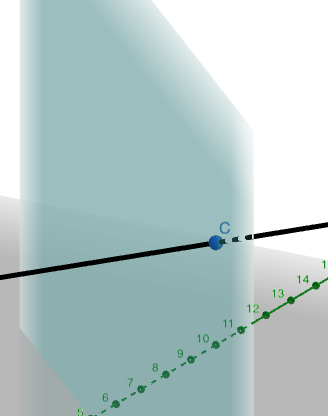
\includegraphics[width=2.5cm]{piano-incotra-retta.png}
        \caption{$E_1 \cap E_2$ è una retta che intersecata con $E_3$ crea un punto}
    \end{subfigure}
    \begin{subfigure}{.3\textwidth}
        \centering
        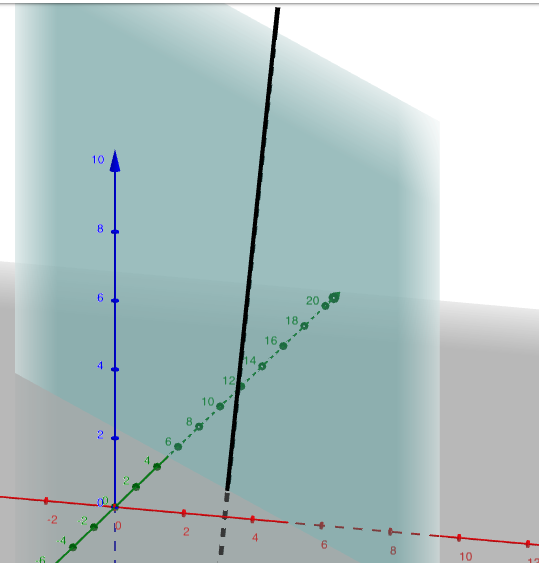
\includegraphics[width=2.5cm]{piano-coincide-retta.png}
        \caption{$E_1 \cap E_2$ può essere contenuto in $E_3$ quindi nuova retta}
    \end{subfigure}
    \begin{subfigure}{.3\textwidth}
        \centering
        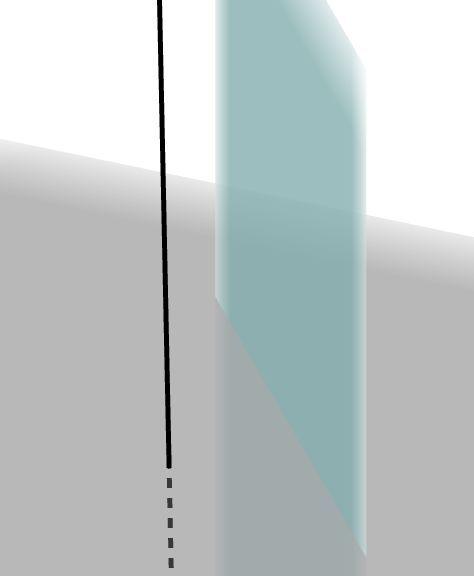
\includegraphics[width=2.5cm]{piano-non-conindice-retta.png}
        \caption{$E_1 \cap E_2$ e $E_3$ possono non coincidere}
    \end{subfigure}
    \caption{Caso 1° esempio}
\end{figure}

\hspace{-15pt}Mentre se vediamo il 2° caso si verifica l'intersezione fra due piani 3 casi come sopra. Mentre un 3° caso è quando c'è l'intersezione con il nulla che rimane nulla.

\subsection{Caso generale}
Possiamo definire un sistema di n equazioni (E) a m variabili con $n,m > 0$ e con $a_{ij}, b{i} \in \mathbb{R}$ come:
\begin{flalign}\nonumber
&E_1: a_{11}x_1 + a_{12}x_2 + ... + a_{1m}x_m = b_1&&\\\nonumber
&E_2: a_{21}x_1 + a_{22}x_2 + ... + a_{2m}x_m = b_2&&\\\nonumber
&\cdots \cdots&&\\\nonumber
&E_n: a_{n1}x_1 + a_{n2}x_2 + ... + a_{nm}x_m = b_n&&\nonumber
\end{flalign}

\begin{definition}[Sistema omogeneo]
Il sistema (E) è \textbf{omogeneo} se $b_1 = ... = b_n = 0$. In caso contrario possiamo considerare il sistema omogeneo associato ($E_{om}$) definito come:
\begin{flalign}\nonumber
&E_1: a_{11}x_1 + a_{12}x_2 + ... + a_{1m}x_m = 0&&\\\nonumber
&E_2: a_{21}x_1 + a_{22}x_2 + ... + a_{2m}x_m = 0&&\\\nonumber
&\cdots \cdots&&\\\nonumber
&E_n: a_{n1}x_1 + a_{n2}x_2 + ... + a_{nm}x_m = 0&&\nonumber
\end{flalign}
\end{definition}

\begin{proposition}\label{prop-1}
Se $(c_1, ..., c_n)$ e $(d_1, ..., d_n)$ sono soluzioni di (E) $\Longrightarrow$ $c_1 - d_1, ..., c_n - d_n$ è soluzione del sistema omogeneo.
\end{proposition}

\begin{demostration}
Se $(c_1, ..., c_n)$ è soluzione vuol dire che :\\
$a_{i1}c_1 + a_{i2}c_2 + a_{im}c_m = b_i$\\
$a_{i1}d_1 + a_{i2}d_2 + a_{im}d_m = b_i$\\
Quindi se sottraggo e raccolgo viene $a_{i1}(c_1 - d_1) + a_{i2}(c_2 - d_m) + a_{im}(c_m - d_m)= 0\:\: \forall \: i,...,n$
\end{demostration}

\begin{theorem}
Se $(c_1,...,c_n)$ è soluzione del sistema (E) tutte le soluzioni (E) sono della forma $(c_1 + e_1, c_2 + e_2, ..., c_m + e_m)$ dove $(e_1,...,e_m)$ è soluzione di $E_{om}$.
\end{theorem}
In sinestesi si può semplificare questo teorema scrivendo:
\begin{equation}
    \text{"Soluzione generale" = "Soluzione particolare" + "Soluzione omogenea"}
\end{equation}

\begin{demostration}
La proposizione \ref{prop-1} dice che le soluzioni hanno questa forma. Viceversa se $(e_1,...,e_m)$ sono soluzioni di ($E_{om}$) $\Longrightarrow$ $(c_1 + e_1, c_2 + e_2, ..., c_m + e_m)$ sono soluzioni di (E).
\end{demostration}

\begin{example}
Prendiamo n=1 e m=2 e prendiamo come sistema di equazioni $(E): 2x + 3y = 5$ e come equazione omogenea $(E_{om}): 2x + 3y = 0$\\\\
Vediamo che le soluzioni particolari sono $x = y = 1$. Per calcolare le soluzioni omogenee si fa $2x = -3y$ e poi $x = -\frac{3}{2}y$, qui per ogni valore di y trovo un valore di x. \\
La soluzioni omogenea è $(-\frac{3}{2}p, p)$ dove p è un parametro che può essere qualsiasi valore.\\
Sappiamo che "sol. generale" = "sol. particolare" + "sol. omogenea" $\Rightarrow (1,1) + (-\frac{3}{2}t,t) = (1 - \frac{3}{2}t, 1 + t)$.
\end{example}

\begin{observation}
$(0,...,0)$ è sempre soluzione di $(E_{om})$. Quindi se (E) ammette una soluzione questo soluzione è unica $\Longleftrightarrow (0,...,0)$ è l'unica soluzione di $(E_{om})$.
\end{observation}

\subsection{Interpretazione geometrica caso generico}
L'interpretazione geometrica per ($E_{om}$) è un "iperpiano attraverso l'origine", e la soluzione è traslazione di questo caso generale per un caso particolare.
\begin{enumerate}
    \item $n=1$, $m=2$ (E) $a_{1n}x_1 + a_{m2}x_2 = b_1$.\\
    Una soluzione $\Longleftrightarrow$ retta ($E_{om}$) $a_1x_1 + a_2x_2 = 0$ una soluzione a (E) $\Rightarrow$ retta attraverso (0,0).
    \item $n=1$, $m=2$, $a_{11}x_1 + a_{12}x_2 + a_{13}x_3 = a$ (E), punto attraverso (0,0,0).
\end{enumerate}

\subsection{Operazioni su (E)}
Per trovare le soluzioni comuni di (E) possiamo usare 3 operazioni per semplificare:
\begin{enumerate}[label=\Alph*]
    \item Scambiare due equazioni.
    \item Moltiplicare $E_i$ per $\lambda \neq 0$ e fare la somma con $E_j$, $E_j \Rightarrow E_j + \lambda E_i$.
    \item Moltiplicare un'equazione $E_i$ per un costate $\lambda \neq 0$, $E_i \Rightarrow \lambda E_i$.
\end{enumerate}

\begin{observation}
Queste operazioni non cambiano l'insieme delle soluzioni di (E) questo perché.
\end{observation}

\begin{demostration}
Dimostriamo le 3 proprietà:
\begin{enumerate}[label=\Alph*]
    \item La prima è ovvia quindi non ha bisogno di una dimostrazione.
    \item Se ($c_1, ..., c_n$) soluzioni di $E_i, E_j \Rightarrow$ anche di $E_i + \lambda E_j$.\\
    Viceversa se ($c_1, ..., c_n$) soluzioni di $E_i$, $E_j + \lambda E_j \Rightarrow$ anche soluzione di ($E_j + \lambda E_i$) - $\lambda = E_j$.
    \item Se ($c_1, ..., c_n$) soluzioni di (E) $\Rightarrow$ anche di $\lambda E$ e viceversa.
\end{enumerate}
\end{demostration}

